\documentclass[
	% parskip=half,
	a4paper,
]{scrarticle}

\usepackage{xcolor}
\definecolor{seeblau}{HTML}{00A9E0}
\definecolor{seegrau}{HTML}{9AA0A7}

\definecolor{seeblau1}{HTML}{CCEEF9}
\definecolor{seeblau2}{HTML}{A6E1F4}
\definecolor{seeblau3}{HTML}{59C7EB}
\definecolor{seeblau4}{HTML}{00A9E0}
\definecolor{seeblau5}{HTML}{008ECE}


\usepackage{graphicx}
\usepackage{amsmath}
\usepackage{subcaption}
\usepackage{wrapfig}
\usepackage[english]{babel}
\usepackage{blindtext}
\usepackage{microtype}
\usepackage{siunitx}
\usepackage[utf8]{inputenc}
\usepackage{csquotes}
\usepackage{nicefrac}
\usepackage[T1]{fontenc}
\usepackage{amsfonts}
\usepackage{amssymb}
\usepackage{tikz}
\usepackage{parskip}

\usepackage{libertinus, libertinust1math}
\usepackage[sfdefault]{biolinum}
\usepackage{roboto}

\setkomafont{disposition}{\normalfont\sffamily}

% set margins
\usepackage{geometry}
\geometry{
	a4paper,
	left=2.5cm,
	right=2.5cm,
	top=2.5cm,
	bottom=2.5cm
}

% caption
\usepackage{caption}
\captionsetup{
	% font={sf},
	labelfont={sf, bf, color=seeblau},
	labelsep=quad,
	labelformat=simple,
}

% links
\usepackage{hyperref}
\hypersetup{
	colorlinks=true,
	linkcolor=seeblau,
	citecolor=seeblau,
	urlcolor=seeblau,
	% hidelinks=true
}

% bibliography
\usepackage[
	style=numeric-comp, % comp = compressed 4,5,6,7 -> 4-7
	sorting=none,		% Sort by appearance
	% autocite = superscript,
	% backref=true,
	hyperref=true,
	url=true,
	maxbibnames=100
]{biblatex}

\usepackage{float}
% \floatplacement{figure}{h}
% \floatplacement{table}{H}

% loosen float placement rules
\renewcommand{\topfraction}{0.8}
\renewcommand{\bottomfraction}{.8}
\renewcommand{\textfraction}{0.1}
\renewcommand{\floatpagefraction}{.9}
% make floats less likely to be placed on a separate page
\setcounter{totalnumber}{9}
\setcounter{topnumber}{9}
\setcounter{bottomnumber}{9}

% decrease space between floats and text
\setlength{\textfloatsep}{0.25cm}
\setlength{\floatsep}{0.25cm}

% decrease space after disposition
\RedeclareSectionCommands[
	afterskip=1px
]{section, subsection, subsubsection}

\usepackage{adjustbox}

\usepackage{datetime}
\newdateformat{dotdate}{
	\twodigit{\THEDAY}.\twodigit{\THEMONTH}.\THEYEAR
}
\newdateformat{monthyeardate}{%
  \monthname[\THEMONTH] \THEYEAR}


% header and footer
\usepackage[
  markcase=noupper
]{scrlayer-scrpage}% activates pagestyle scrheadings automatically
\clearpairofpagestyles
\setkomafont{pageheadfoot}{\normalfont\sffamily}
\setkomafont{pagenumber}{\normalfont\sffamily}
% \chead*{\color{seegrau} Draft \dotdate\today}
\ofoot*{\pagemark}
\ohead*{\rightmark}


\usepackage{ifthen}
\newcommand{\markieren}[4]{
	\ifthenelse{\equal{#1}{}}{}{\adjustbox{padding=3pt, bgcolor=seeblau1, margin=-1pt}{\strut{\sffamily\robotoMedium{#1}}}\\}
  \ifthenelse{\equal{#2}{}}{}{\adjustbox{padding=3pt, bgcolor=seeblau2, margin=-1pt}{\strut{\sffamily\robotoMedium{#2}}}\\}
	\ifthenelse{\equal{#3}{}}{}{\adjustbox{padding=3pt, bgcolor=seeblau3, margin=-1pt}{\strut{\sffamily\robotoMedium{#3}}}\\}
	\ifthenelse{\equal{#4}{}}{}{\adjustbox{padding=3pt, bgcolor=seeblau4, margin=-1pt}{\strut{\sffamily\robotoMedium{#4}}}}
}

\addbibresource{../literature.bib}
\begin{document}

\author{Leon Oleschko}
\date{\dotdate\today}

\begin{titlepage}
    \sffamily
    \vspace*{3cm}
    {
        \fontsize{32}{32}
        \markieren{Ultrafast}{Photoluminescence}{from Thermal}{Radiation}
        % \title{Ultrafast Photoluminescence}
    }
    \vspace{.25cm}\\
    {
        \Large
        Leon Oleschko\\
        supervised by Peter Baum
        \vspace{.05cm}\\
        \dotdate\today\\
        \textbf{Draft}\\
        \vspace{.05cm}\\
        \normalsize
        Projekt Praktikum\\
        Universität Konstanz
    }
    \vfill
    {
        \normalfont\normalsize
    }
    \vfill
    \begin{flushright}
        Available at \url{www.github.com/leoole100/projekt-praktikum}.
    \end{flushright}
\end{titlepage}

% {
% 	\sffamily
% 	\hypersetup{hidelinks}
% 	\tableofcontents
% }

\clearpage

\section{Introduction}


\clearpage
\section{Numerical Model}

\begin{figure}[b]
    \centering
    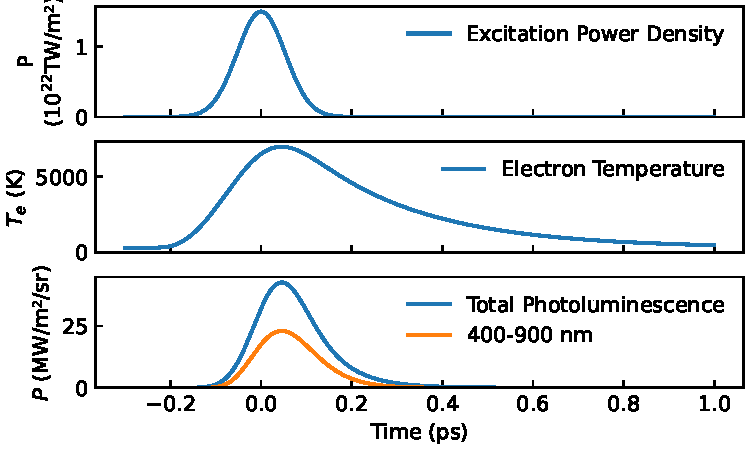
\includegraphics{../analysis/figures/model.time_evolution.pdf}
    \caption{Time evolution of the absorbed power density $P_V(t)$, the electron temperature $T_e(t)$ and the total integrated radiance $L(t)$, calculated using the two-temperature model (Eq. \ref{eq:Te}). The calculation assumes an absorbed energy density of $U_{\text{abs}} = \SI{2e9}{J/m^3}$ over a FWHM pulse with $t=\SI{250}{fs}$ and an electron-phonon coupling time of $\tau=\SI{250}{fs}$ (for graphite). The rapid temperature rise and subsequent decay illustrate the ultra-fast nature of the thermal dynamics.}
    \label{fig:timeevolution}
\end{figure}

The ultrafast thermal dynamics are modeled using a simplified two-temperature approach. An excitation pulse $P_{\text{exc}}(t)$ generates an absorbed power density $P_V(t) = P_{\text{exc}}(t) / V$ over the material's volume $V$. This input energy raises the electron temperature $T_e$, governed by the electronic heat capacity $C_e(T_e)$. Subsequently, the electrons cool via electron-phonon coupling with a relaxation time $\tau$ to the lattice at a constant temperature $T_l$.

This process is described by the ordinary differential equation:
\begin{equation}
    \frac{\mathrm d T_e(t)}{\mathrm d t}
    =
    \frac{P_V(t)}{C_e(T_e)}
    -\frac{T_e(t) - T_l}{\tau}.
    \label{eq:Te}
\end{equation}
A numerical solution based on used excitation parameters (an absorbed energy density of $U_{\text{abs}} = \SI{2}{GJ/m^3}$ spread in a Gaussian pulse with a full width at half maximum (FWHM) of $\SI{250}{fs}$) is provided. We utilize the electronic heat capacity function from \cite{nihiraTemperatureDependenceLattice2003} and the $\tau=\SI{250}{fs}$ coupling time for graphite \cite{stangeHotElectronCooling2015}. The resulting time evolution is shown in \autoref{fig:timeevolution}.

The spectral radiance $L_\lambda$ emitted at each time step can be calculated using Planck's law:
\begin{equation}
    L_\lambda(\lambda,T)
    = \epsilon(\lambda) \frac{2hc^{2}}{\lambda^{5}}
    \frac{1}{\exp\bigl(hc / \lambda k_{\mathrm B}T\bigr)-1}.
\end{equation}
The electron gas emissivity $\epsilon$ is assumed to be unity, a common approximation for graphite \cite{sapritskyBlackbodyRadiometry1995}. The resulting time evolution of the total radiance $L=\int L_\lambda(\lambda, T) d\lambda$ and the radiance in a spectral range relevant for common detectors are also presented in \autoref{fig:timeevolution}.

\begin{figure}
    \centering
    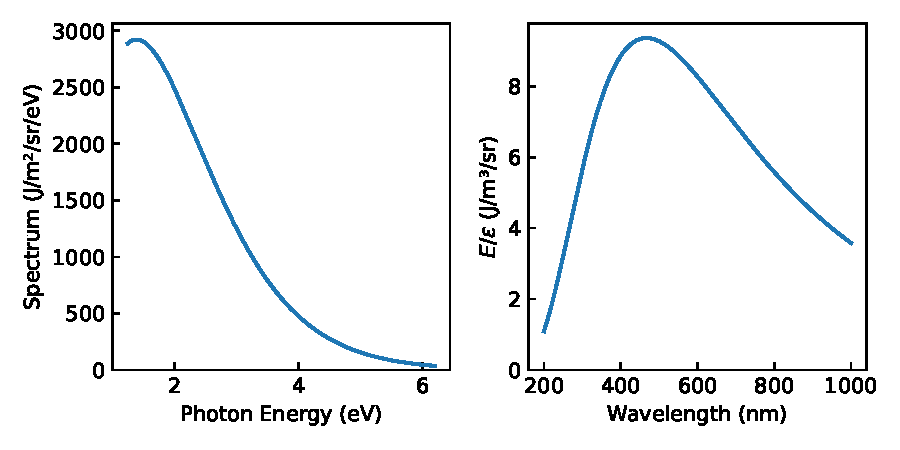
\includegraphics{../analysis/figures/model.spectrum.pdf}
    \caption{Model spectrum $H_\lambda(\lambda)$ (time-integrated spectral radiance) calculated from the time evolution shown in Figure \ref{fig:timeevolution}. The spectrum represents the total signal expected to be recorded by a time-integrating detector. Both shown over the wavelength and the photon energy.}
    \label{fig:model_spectrum}
\end{figure}

The experimentally measurable spectrum, $H_\lambda(\lambda)$, is defined as the time-integrated spectral radiance:
\begin{equation}
      H_\lambda(\lambda) = 
      \int L_\lambda\bigl(\lambda, T_e(t)\bigr)\,\mathrm dt.
\end{equation}
This is shown in \autoref{fig:model_spectrum}. It is noted that this spectrum can alternatively be visualized as a function of photon energy $E = h c / \lambda$. For direct comparison with the spectrometer output, however, we opt for the wavelength representation in this report.

\subsection{Sensitivity}

\begin{figure}
    \centering
    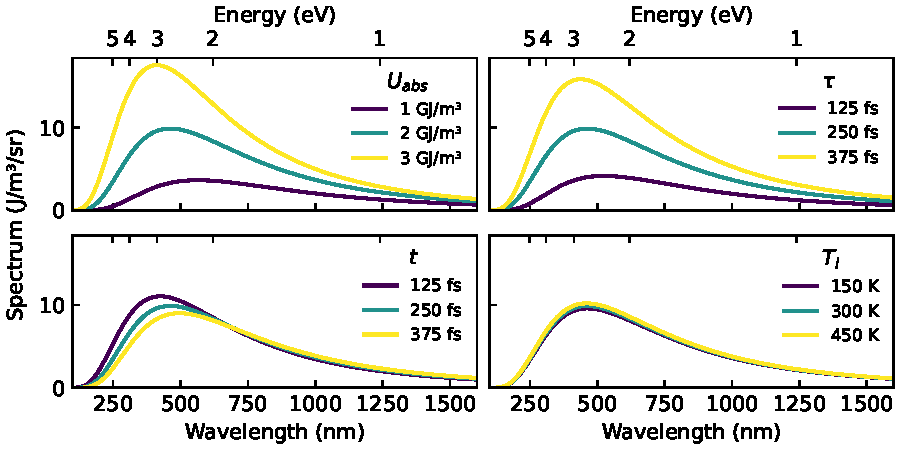
\includegraphics{../analysis/figures/sensitivity.pdf}
    \caption{Sensitivity analysis of the calculated spectrum $H_\lambda(\lambda)$ to changes in key model parameters. The results demonstrate that the absorbed energy density $U_{\text{abs}}$ and the electron-phonon coupling time $\tau$ are the dominant factors influencing the spectral shape and total emission. Conversely, variations in the pulse duration $t$ and the lattice temperature $T_l$ show only marginal impact.}
    \label{fig:sensitivity}
\end{figure}
This model is employed to study the sensitivity of the resulting spectrum to changes in the defining physical and experimental parameters. The spectrum is calculated while systematically sweeping each parameter, as detailed in \autoref{fig:sensitivity}.

The analysis reveals that the spectrum changes considerably with variations in the absorbed energy density $U_{\text{abs}}$ and the electron-phonon coupling time $\tau$. This high sensitivity emphasizes the critical importance of precisely controlling these two parameters. In contrast, changes in the excitation pulse duration $t$ and the lattice temperature $T_l$ do not significantly alter the resulting spectrum.

\begin{figure}
    \centering
    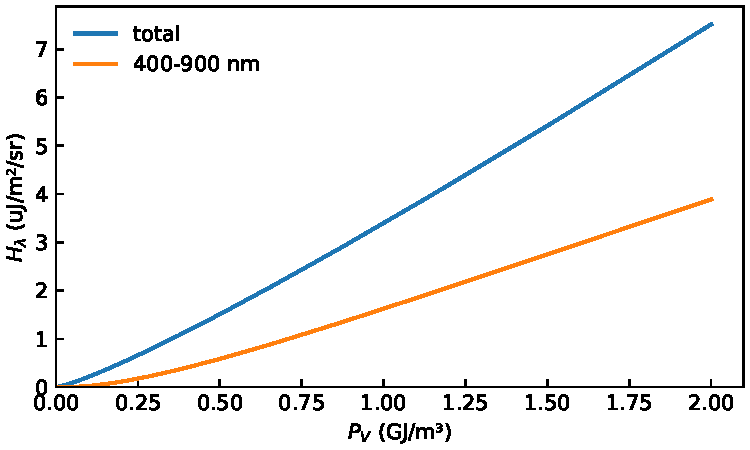
\includegraphics{../analysis/figures/powerscaling.pdf}
    \caption{Scaling behavior of the emitted thermal radiation as a function of the absorbed energy density $U_{\text{abs}}$. The scaling is shown for both the total integrated spectrum ($\int H_\lambda d\lambda$) and the radiance within the detector's spectral region. Note the non-power-law dependence, which stems from the temperature-dependent electronic heat capacity $C_e(T_e)$.}
    \label{fig:powerscaling}
\end{figure}
The dependence of the total emitted power $\int H_\lambda(\lambda) d\lambda$ on the absorbed energy density is shown in more detail in \autoref{fig:powerscaling} for both the total emission and the spectral range relevant for the detector.

Crucially, the scaling is not described by a simple power law. This non-trivial behavior is a direct consequence of the changing electronic heat capacity $C_e(T_e)$ at high temperatures.

\clearpage
\section{Experimental Setup}
\begin{figure}[h]
    \centering
    \begin{subfigure}{3.5in}
        \centering
        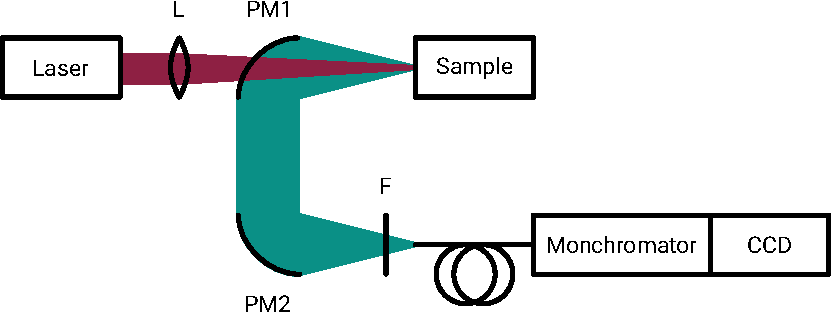
\includegraphics{figures/setup.pdf}
        \caption{Schematic}
    \end{subfigure}\hfill
    \begin{subfigure}{2in}
        \centering
        \includegraphics{figures/photo_setup.pdf}
        \caption{Photograph}
    \end{subfigure}
    \caption{Experimental setup used to measure thermal emission from ultrafast-excited hot electrons. The schematic shows the optical path and key components; the photograph shows the arrangement inside the chamber.}
    \label{fig:setup}
\end{figure}

The experimental setup, originally developed by Leon Roob~\cite{roobThermalRadiationUltrafast2025}, is shown in \autoref{fig:setup}. It is designed to measure broadband thermal emission from hot electrons in graphite using reflective collection optics and a fibre-coupled spectrometer.

The excitation source is a PHAROS PH1-20 (Light Conversion) at a centre wavelength of \SI{1030}{\nano\metre}, with pulse duration \SI{250}{\femto\second} (FWHM) and repetition rate \SI{40}{\kilo\hertz}. The pulse energy is \SI{7.5}{\micro\joule} (average power \SI{300}{\milli\watt}). The beam is stabilised in four axes and expanded to a diameter of $D=\SI{5}{\milli\metre}$ before entering the chamber.

Inside the chamber, a plano-convex lens with focal length \(f=\SI{200}{\milli\metre}\) focuses the beam onto the sample. Using the standard diffraction estimate \(d \approx 4\lambda f / \pi D\), the spot diameter is \(\SI{50}{\micro\metre}\).

The target is a graphite sample mounted on a three-axis translation stage. Thermal emission from the irradiated spot is collected by two off-axis parabolic mirrors (UV-enhanced aluminium). The first mirror (PM1, \(f=\SI{50}{\milli\metre}\)) collimates the emission; the second (PM2, \(f=\SI{101}{\milli\metre}\)) focuses it onto a band-pass filter and into a multimode fibre with a \SI{200}{\micro\metre} core (Ocean Optics QP200-2-SR-BX). The magnification is \(M = f_{\mathrm{PM2}}/f_{\mathrm{PM1}} \approx 2\), yielding an image spot of \(\sim\SI{100}{\micro\metre}\) at the fibre entrance, comfortably within the core.

The fibre feeds an Acton SpectraPro 300i monochromator equipped with a 150\,lines\,mm\(^{-1}\) grating blazed at \SI{500}{\nano\metre}. The dispersed spectrum is detected by an Andor iXon\textsuperscript{EM}+ 897 EMCCD operated in vertical binning mode, effectively serving as a 1D line detector.
Wavelength calibration (performed once following the manufacturer’s procedure~\cite{roobThermalRadiationUltrafast2025}) was stable throughout the measurements.

For alignment and maximal throughput, the lens, sample, and fibre ferrule are mounted on independent precision translation stages, while PM1 and PM2 are fixed on the common optical axis. 

\subsection{Noise and detector considerations}
Detecting the weak thermal radiation from hot electrons requires careful optimisation of the signal-to-noise ratio (SNR). In this setup the dominant noise sources originate from the detector; laser power fluctuations and mechanical variations are treated as negligible. The EMCCD mechanisms are well documented by Andor~\cite{dr.jowaltersSensitivityNoiseCCD2023,andorEstablishingSensitivityScientifica} and standards \cite{europeanmachinevisionassociationStandardCharacterizationImage2010}.

\textbf{Readout noise.}
This is the fundamental noise from charge transfer and A/D conversion. For the present camera, the fit in \autoref{fig:dark_noise} yields a constant read noise of
\(\sigma_{\text{read}}=\SI{0.81(12)}{DN}\), consistent with the manufacturer’s specification~\cite{andorIXonEM897Manual}.
Because read noise is applied per read out bin, hardware binning (1D line-detector mode) reduces its impact by summing signal prior to the single read.

\textbf{Dark current noise.}
Thermally generated charge scales with temperature and time,
\(N_\text{dark}\propto \exp(-E/kT)\,t_\text{exp}\).
\autoref{fig:dark_noise} shows the measured dependence; fitting gives an effective activation energy \(E=\SI{0.597(4)}{eV}\).
With the sensor cooled to \SI{-80}{\degreeCelsius}, the dark contribution is negligible at the exposure times used.

\begin{figure}[h]
    \centering
    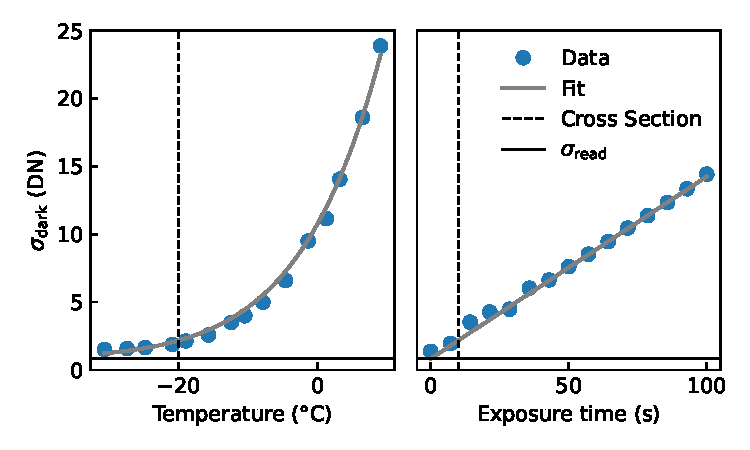
\includegraphics{../analysis/figures/dark_noise.pdf}
    \caption{Dark noise vs.\ sensor temperature and exposure time. Fit yields \(E=\SI{0.597(4)}{eV}\) and \(\sigma_{\text{read}}=\SI{0.81(12)}{e^{-}}\).}
    \label{fig:dark_noise}
\end{figure}

\textbf{Clock-induced charge (CIC).}
CIC is created during high-speed clocking.
Its apparent contribution grows with electron multiplication gain, so \emph{EM gain is disabled} in this work (signal levels are well above the read-noise floor), which keeps CIC negligible~\cite{andorEstablishingSensitivityScientifica}.

\textbf{Shot noise and photon-transfer method.}
Under these optimised conditions the dominant term is shot noise.
Incident photons create photoelectrons with quantum efficiency \(\eta\), so \(N_e=\eta\,N_{\text{photons}}\) and, for Poisson statistics, \(\operatorname{var}(N_e)=N_e\)~\cite{europeanmachinevisionassociationStandardCharacterizationImage2010}.
Let \(G\) denote the system conversion gain (DN per electron). The measured signal in data numbers (DN) is \(S = G\,N_e\), and the measured variance becomes \(\sigma^2_{\text{meas}} \;=\; \sigma_{\text{read}}^2 \;+\; G\,S\).
Thus a plot of variance vs.\ mean (photon-transfer curve) is linear in the shot-noise regime with slope \(G\).
\autoref{fig:shotnoise} shows this behaviour; from the slope \(G \approx 10~\text{DN}/e^{-}\) can be measured.
Note that this procedure does \emph{not} determine \(\eta\); it only gives the DN-to-electron conversion.

\begin{figure}[h]
    \centering
    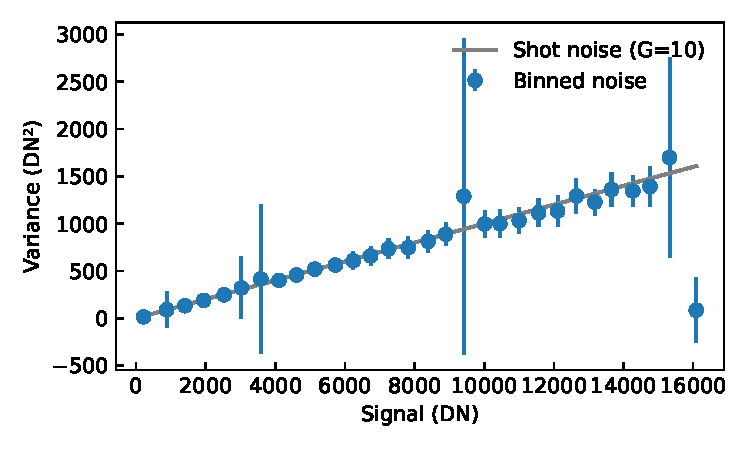
\includegraphics{../analysis/figures/shot noise.pdf}
    \caption{Measured noise vs.\ signal (photon-transfer curve) demonstrating shot-noise-limited operation; the linear slope yields the conversion gain \(G\).}
    \label{fig:shotnoise}
\end{figure}

\subsection{Data processing}
All raw spectra were first corrected by subtracting a dark frame recorded with identical acquisition settings, removing the fixed electronic bias and dark current.  
Residual peaks at the fundamental and harmonic wavelengths of the pump laser, normally suppressed by laser line filters, were present due to the absence of suitable optical filtering.  
These peaks were identified and removed digitally, leaving gaps in the plotted spectra where the affected bins were excluded.  

The corrected signal \(S(\lambda)\) in DN was converted to spectral power density \(P_{\text{meas}}(\lambda)\) via
\begin{equation}
  P_{\text{meas}}(\lambda)
  = \frac{S(\lambda)}{G\,t_{\text{exp}}\,\Delta\lambda}\,\frac{hc}{\lambda},
\end{equation}
with \(G\) the DN/\(e^-\) conversion gain, \(t_{\text{exp}}\) the exposure time, and \(\Delta\lambda\) the spectral bin width.  

\clearpage
\section{Measurement}
\begin{figure}[h]
    \centering
    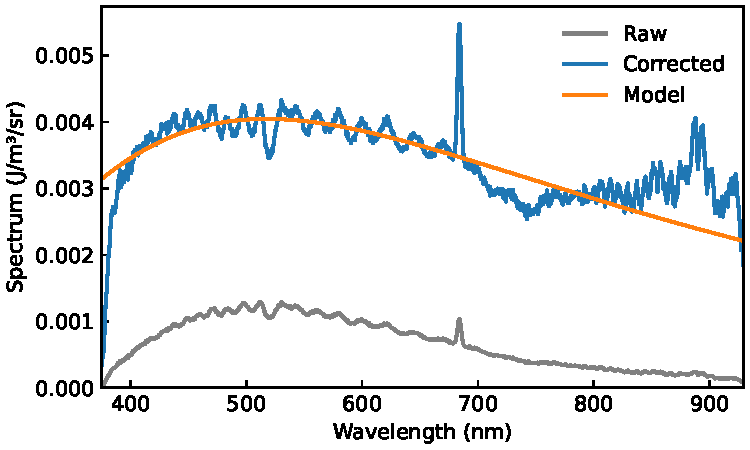
\includegraphics{../analysis/figures/combined.fit.pdf}
    \caption{}
    \label{fig:fit}
\end{figure}
\begin{figure}
    \centering
    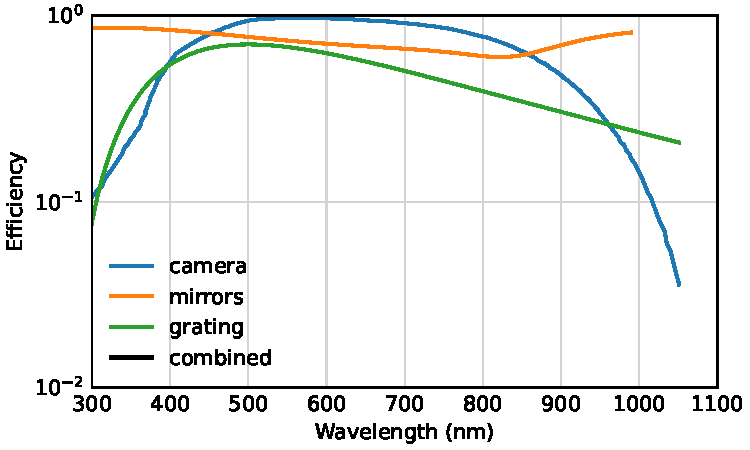
\includegraphics{../analysis/figures/combined.efficiency.pdf}
    \caption{}
    \label{fig:efficiency}
\end{figure}
Before comparing the model with the measurement, the raw measurement (shown in \autoref{fig:fit}) has to be corrected with the instruments calibration curve.
This contains the manufacturer supplied efficiency of the camera \cite{andorIXonEM897Manual} and the efficiency curve of the monochromator.
This is modelled using \autocite{barkerRippleCorrectionHighdispersion1984} and the unknown model parameter $k=1.18$ is fitted by minimizing the error between the corrected spectrum and the model.
The model and the fitted corrected spectrum is also shown in \autoref{fig:fit}.
The model is scaled by \SI{0.72e-3}{} and the absorbed energy density $U_\text{abs} = \SI{1.35}{GJ/m^3}$ fitted to the measurement.

The vastly different scale of the model to the measurement was later attributed to a defective coupling of the fiber to the spectrometer, with a loss in the order of $10^3$. 
The incident energy density $U_\text{inc} = P_\text{avg} \; / \; f_\text{rep} \pi r_\text{spot}^2 d = \SI{4.8e9}{J/m^3}$ with the average Power $P_\text{avg}=\SI{300}{mW}$, the repetition rate $f_\text{rep}=\SI{40}{kHz}$, the spot size $r_\text{spot}=\SI{50}{\micro m}$ and the absorption depth $d=\SI{200}{nm}$ \cite{smauszDeterminationUVVisible2017} is more due to some light being reflected and scattered. It correspondence with a incident fluence of \SI{950}{J/m^2}. 

The light around \SI{900}{nm} and the peak at peak at \SI{688}{nm} in the corrected spectrum may be due to the laser light not being filtered before reaching the sample.

\section{Discussion and Conclusion}

\clearpage
\printbibliography

\end{document}